\chapter{Proposed implementation}\label{chap:proposal}
In this chapter, we are going to describe the implementation we propose, the technologies we intend to use and the models we aim to examine.


\section{Technologies}
In this thesis, we implement all of the studied models in python deep learning library Keras with Tensorflow backend. All of the experiments are conducted on NVIDIA GTX 1070.

% ...Software, frameworks, libraries to be used... GPU used
\section{Benchmark datasets}

In this section, we are going to describe the datasets which will be used for the evaluation purposes of this thesis. All of the datasets mentioned below were made publicly available for research purposes.
\subsection{ITOP}
The Invariant-Top View Dataset (ITOP) \cite{haque2016viewpoint} consists of approximately 50k real-world depth images from two camera viewpoints (front view and top view). It captures 20 people, each performing 15 different actions. The dataset comes with the initial partition of the data into the train and test set. The train and test data contain around 18k and 5k samples from each viewpoint, respectively. Besides the depth images and the ground-truth joint labels, the dataset also includes raw point clouds. The skeletal model in this dataset is described by 15 body joints. Sample depth maps from the dataset are shown in Fig. \ref{fig:itop}. As can be seen in the figure, the depth images are rather noisy, but the noise can be partly reduced by several background segmentation methods.\par

\vspace{5mm}
\begin{figure}[H]
\begin{center}
  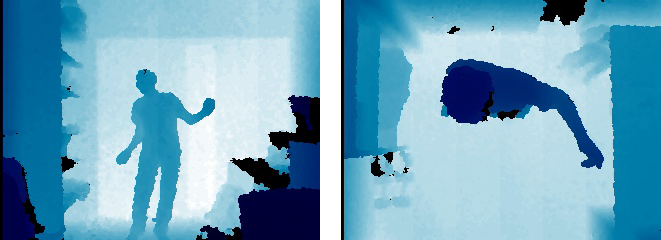
\includegraphics[height=130px]{images/implementation/itop.png}
  \caption[Sample depth images from the ITOP dataset \cite{haque2016viewpoint}.]{Sample depth images from the ITOP dataset \cite{haque2016viewpoint} (front and top view).}
  \label{fig:itop}
\end{center}
\end{figure}

\noindent
The current state-of-the-art on ITOP dataset was claimed in \cite{Marin18jvcir}, where the 100\% accuracy at 10cm precision was reached, which means every joint was predicted within 10cm from its ground-truth position. In the paper, they also claim to have reached the mean error of approximately 0.9cm on ITOP dataset (0.19cm on the front-view data), which is the best result achieved on the stated dataset, up to our knowledge.

\subsection{UBC3V}

The UBC3V \cite{Shafaei16} is a synthetic dataset made for the task of pose estimation from multiple cameras. It contains around 6 million synthetic depth frames structured in three parts according to the complexity of the human postures – easy, medium and hard pose. The pose in each frame is represented by the position of 18 skeletal joints. It captures a total of 16 characters and each frame is observed from three different viewpoints. Thus, the samples can be treated both as multi-view (point clouds from three cameras merged into one), or single-view postures (each sample handled separately). Although the multi-view point clouds describe a particular posture in a more complex way, considering the use-case in most of the real-time applications, the single-view samples are often the preferred option, due to the difficulty of the task of multiple camera synchronization.\par

\vspace{5mm}
\begin{figure}[H]
\begin{center}
  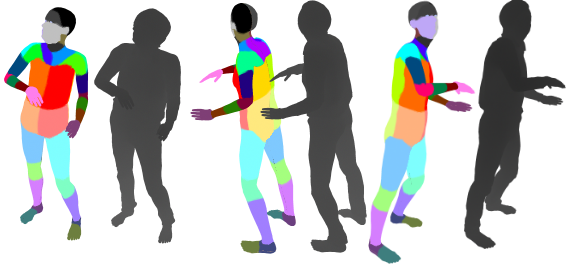
\includegraphics[height=130px]{images/implementation/ubc3v.png}
  \caption[Sample data from the UBC3V dataset \cite{Shafaei16}.]{Sample data from the UBC3V dataset (the figure shows the same pose from three different cameras) \cite{Shafaei16}.}
  \label{fig:ubc3v}
\end{center}
\end{figure}

\noindent
 The depth data are available in the form of depth images, but can be converted into point clouds in world reference coordinates using the intrinsic and extrinsic camera parameters. The ground truth labels are composed of 18 joints per posture, and the dataset also comprises a segmentation of each point cloud into 43 body regions (as can be seen in Fig \ref{fig:ubc3v}).

\subsection{MHAD}
The Berkeley Multimodal Human Action Database (MHAD) \cite{Vidal:2013:BMC:2478277.2478412} was recorded on real humans. It contains 11 actions performed by 7 male and 5 female subjects. Each subject performed each of the actions 5 times, which yields about 660 action sequences corresponding to about 82 minutes of total recording time. The total number of depth frames is over 250k. The skeleton structure in this dataset is defined by 35 joint locations. Two of the performed actions involve a chair, used for the subject to sit down and stand up. It is worth a mention, that the chair itself provides a lot of clutter in the depth data. The whole dataset was captured by multiple devices, including cameras, depth sensors, accelerometers and microphones. Two kinect cameras were used and synchronized to acquire the depth data, one placed in front of the subject, the other one at the back. Intrinsic and extrinsic camera parameters are provided to extract the scene as a point cloud with real-world coordinates.\par

\subsection{CMU Panoptic Dataset}
\cite{Joo_2017_TPAMI}

%\subsection{PKU-MMD}  % ? TODO  

%\subsection{Novel dataset} 
\section{Approaches}
... different approaches implemented + novel proposed method - two-stage pipeline Four-channel Pose Estimation ...


\subsection{Deep Depth Pose model}
One of the aims of this work, is to implement the Deep Depth Pose model (DDP) \cite{Marin18jvcir} in Keras framework. We consider this an essential step to propose a state-of-the-art pose estimation model performing on depth data, since the DDP model claims to outperform all of the present methods on the examined datasets.\par
\vspace{5mm}
\noindent
Originally, the model is implemented in Matlab and while some parts of the code (mostly testing) are publicly available, the training procedures were not published. 

\subsection{Point-Based Pose Estimation model}

% TODO toto cele uz do proposed implementation, potom v implementation uz implementacne detaily, preprocessing dat, upravy modelu, ... 
...\newline
In the model he proposed, instead of the first (segmentation) stage, he made use of the auxiliary sub-network, which computes the body-part segmentation on the fly, while the main network regresses the joint locations. The whole architecture of the stated model is shown in Fig. \ref{fig:PBPE}. \par
\vspace{5mm}
\begin{figure}[H]
\begin{center}
  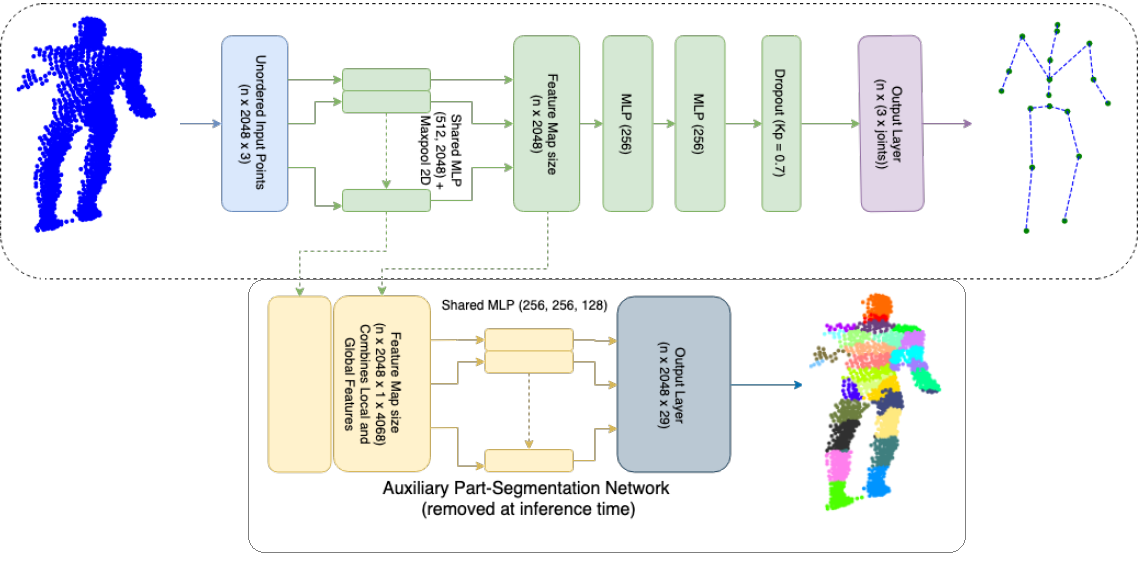
\includegraphics[height=200px]{images/related_work/pbpe2.PNG}
  \caption{The Point-Based Pose Estimation model architecture \cite{Ali19}.}
  \label{fig:PBPE}
\end{center}
\end{figure}

\noindent The basic idea behind the structure of the model is the aggregation of both local and global features of the input point cloud in the auxiliary part-segmentation network. Without the sub-network, almost all of the local context would be lost because of the max-pooling aggregation in the intermediate layers. Thanks to the incorporation of the local features, the network can better understand the relationships among particular local regions of the human body.\par
\vspace{5mm}


\subsection{Four-channel Pose Estimation}


%\begin{minipage}{\textwidth}
%	Sily v našom modeli možno rozdeliť do dvoch skupín:
%	\begin{itemize}
%		\item interné sily
%		\item externé sily
%	\end{itemize}
%\end{minipage}\newline




